%!TEX root = ../nips_2017.tex


\begin{figure}[t]
    \centering
     \subfigure[$K=10$, $L=32$.]{
     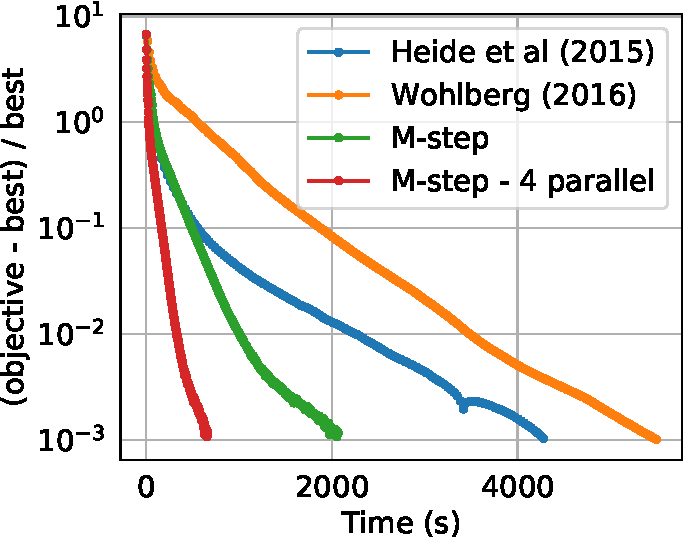
\includegraphics[width=0.30\linewidth]{figures/relative_10_32.pdf}}
     \subfigure[Time to reach a relative precision of 0.01.]{
     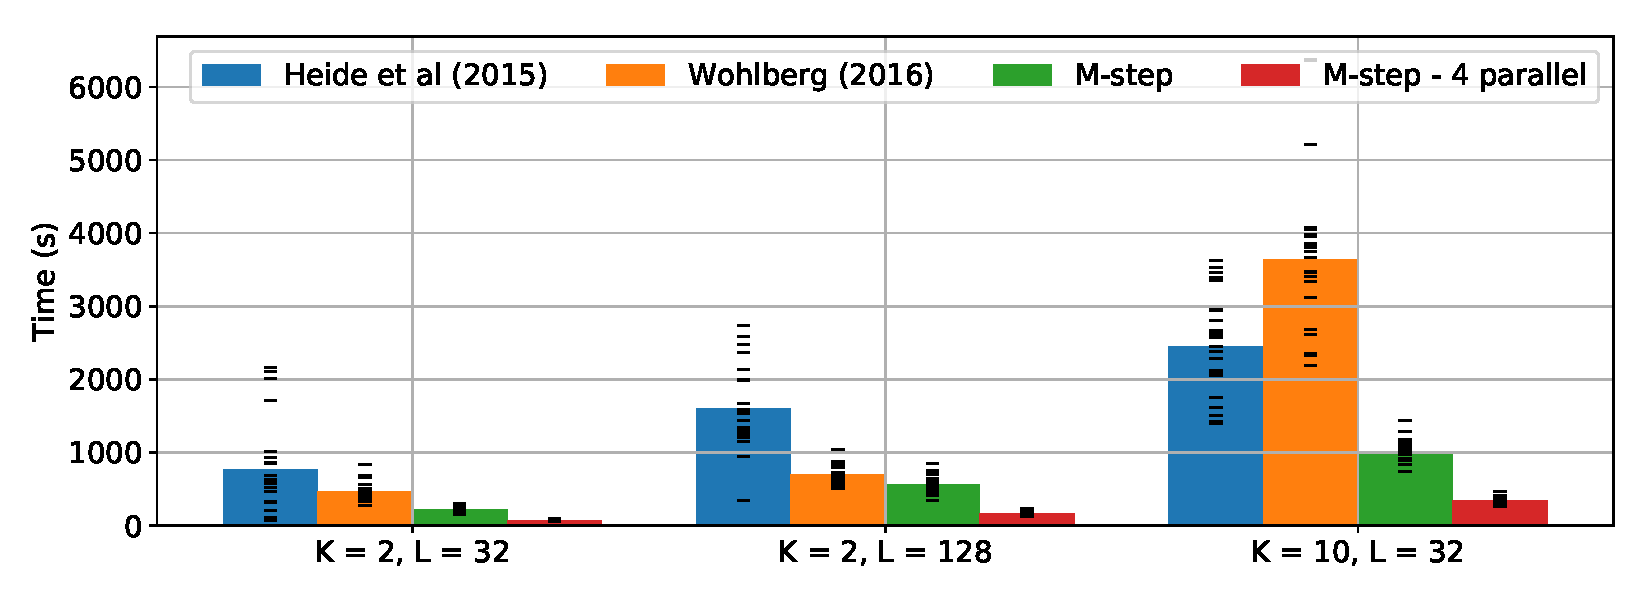
\includegraphics[width=0.67\textwidth]{figures/bar_plot.pdf}}
    \vspace{-10pt}
    \caption[Comparison of state-of-the-art methods with our approach.]{Comparison of state-of-the-art methods with our approach. (a)~Convergence plot with the objective function relative to the obtained minimum, as a function of computational time. (b)~Time taken to reach a relative precision of $10^{-2}$, for different settings of $K$ and $L$.  }
    \label{fig:convergence}
\end{figure}

\section{Experiments}
\label{sec:experiments}
In order to evaluate our approach, we conduct several experiments on both synthetic and real data. 
First, we show that our proposed optimization scheme for the M-step provides significant improvements in terms
of convergence speed over the state-of-the-art CSC methods. Then, we provide empirical evidence that our algorithm is more robust to
artifacts and outliers than three competing CSC methods~\cite{jost2006motif,brockmeier2016learning,wohlberg2016efficient}.
%
Finally, we consider LFP data, where we illustrate that our algorithm can reveal interesting properties in electrophysiological signals
without supervision, even in the presence of severe artifacts. The source code is publicly available at \url{https://alphacsc.github.io/}.


% We then show that our algorithmic strategy based on temporal convolutions
% and L-BFGS-B for the M-step outperforms state-of-the-art solvers in terms
% of convergence speed. 



% \paragraph{Synthetic simulation setup:}
\textbf{Synthetic simulation setup:} 
In our synthetic data experiments, we simulate $N$ trials of length $T$ by first generating $K$ zero mean and unit norm atoms of length $L$. The  activation instants are integers drawn from a uniform distribution in $\llbracket0, T-L \rrbracket$. The amplitude of the activations are drawn from a uniform distribution in $[0, 1]$. Atoms are activated only once per trial and are allowed to overlap. The activations are then convolved with the generated atoms and summed up as in \eqref{eq:problem_definition}. 


% \paragraph{M-step performance:}
\textbf{M-step performance:} 
In our first set of synthetic experiments, we illustrate the benefits of our M-step optimization approach over state-of-the-art CSC solvers. 
%
%Besides existing CSC solvers cannot be directly applied to the M-step of our algorithm for $\alpha < 2$, even in the case where $\alpha=2$ they turn out to be not as efficient when applied to neural signals, since they solve the problem in the Fourier domain which introduces additional projection operations. 
%
We set $N=100$, $T=2000$ and $\lambda=1$, and use different values for $K$ and $L$. To be comparable, we set $\alpha=2$ and add Gaussian noise to the synthesized signals, where the standard deviation is set to $0.01$. In this setting, we  have $w_{n,t}=1/2$ for all $n$, $t$, which reduces the problem to a standard CSC setup. We monitor the convergence of ADMM-based methods by \citet{heide2015fast} and \citet{wohlberg2016efficient} against our M-step algorithm, using both a single-threaded and a parallel version for the $z$-update. 
% We used here artifact-free data. 
As the problem is non-convex, even if two algorithms start from the same point, they are not guaranteed to reach the same local minimum\footnote{Note that the M-step can be viewed as a biconvex problem, for which global convergence guarantees can be shown under certain assumptions \cite{agarwal2014learning, gorski2007biconvex}. However, we have observed that it is required to use multiple restarts even for vanilla CSC, implying that these assumptions are not satisfied in this particular problem.}. 
%
Hence, for a fair comparison, we use a multiple restart strategy with averaging across $24$ random seeds.




 % we observe that in practice, the sampling route does not come with any additional disadvantage due to our multiple restart strategy.

% It is true that the vanilla CSC can be viewed as a biconvex problem with guarantees for convergence to the global minimum under some assumptions (e.g., Agarwal et al, 2014; Gorski et al, 2007). However, we observe in practice that these assumptions are not satisfied, which is why we need to use multiple restarts even for vanilla CSC. Therefore, in introducing an EM loop, we do not sacrifice such convergence properties.

% the d-updates for

During our experiments we have observed that the ADMM-based methods do not guarantee the feasibility of the iterates. In other words, the norms of the estimated atoms might be greater than $1$ during the iterations. To keep the algorithms comparable, when computing the objective value, we project the atoms to the unit ball and scale the activations accordingly. To be strictly comparable, we also imposed a positivity constraint on these algorithms. This is easily done by modifying the soft-thresholding operator to be a rectified linear function. In the benchmarks, all algorithms use a single thread, except ``M-step - 4 parallel'' which uses 4 threads during the $z$ update.

In Fig.~\ref{fig:convergence}, we illustrate the convergence behaviors of the different methods.
%Note that the y-axis is the relative precision with respect to the best obtainable objective function value upon convergence for the local minima that the algorithm converges to. % nice one !
Note that the y-axis is the precision relative to the objective value obtained upon convergence. In other words, each curve is relative to its own local minimum (see supplementary document for details).
In the right subplot, we show how long it takes for the algorithms to reach a relative precision of $0.01$ for different settings (\textit{cf.} supplementary material for more benchmarks). Our method consistently performs better and the difference is even more striking for more challenging setups. This speed improvement on the M-step is crucial for us as this step will be repeatedly executed. % in the EM algorithm. 
%This sets the stage for us to apply $\alpha$CSC on datasets of realistic dimensions.
%
\newcommand{\tmpsize}{0.14}
\begin{figure}[t]
%\vskip 0.2in
\begin{center}
\vspace{-10pt}
\subfigure[No corruption.]{
 \setlength{\tabcolsep}{0.5pt} 
    \begin{tabular}{c c}

        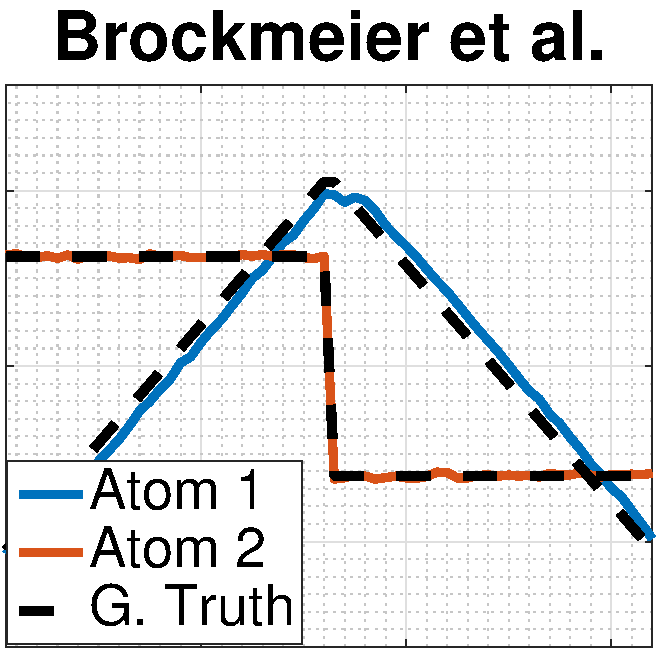
\includegraphics[width=\tmpsize\linewidth]{figures/synth_1_rnn_v2.pdf} &
        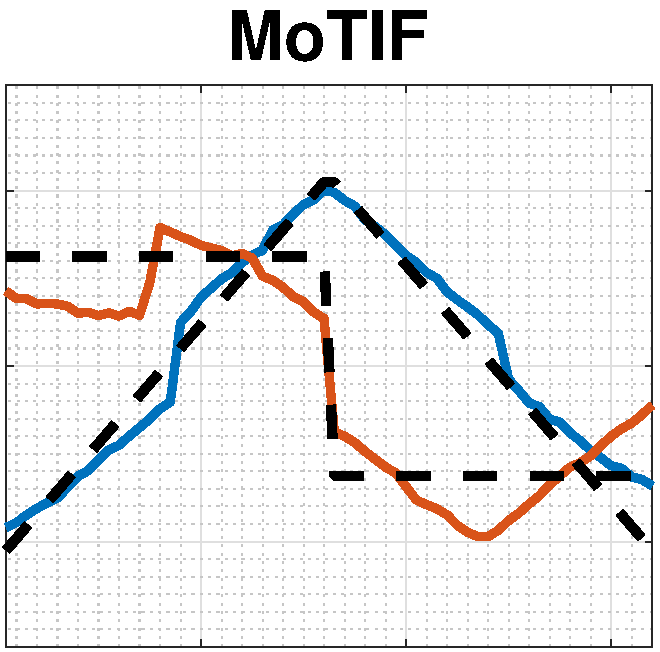
\includegraphics[width=\tmpsize\linewidth]{figures/synth_1_motif_v2.pdf}
        \\
        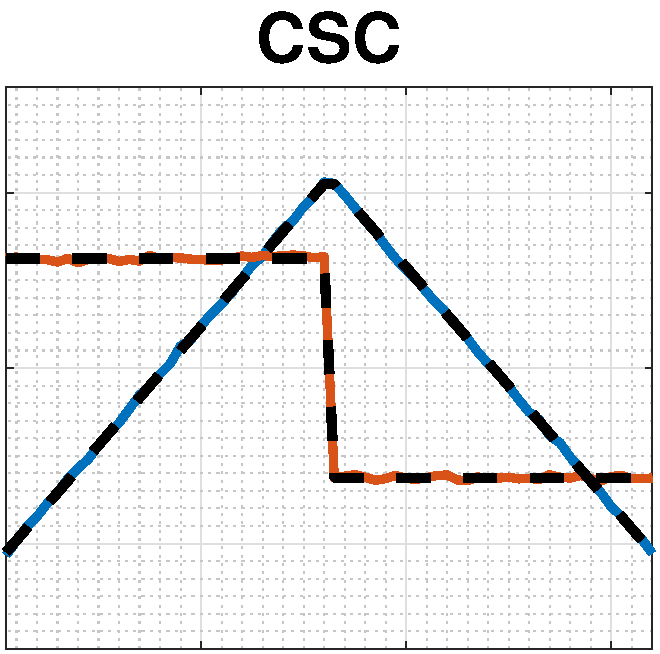
\includegraphics[width=\tmpsize\linewidth]{figures/synth_1_1_v2.pdf} &
        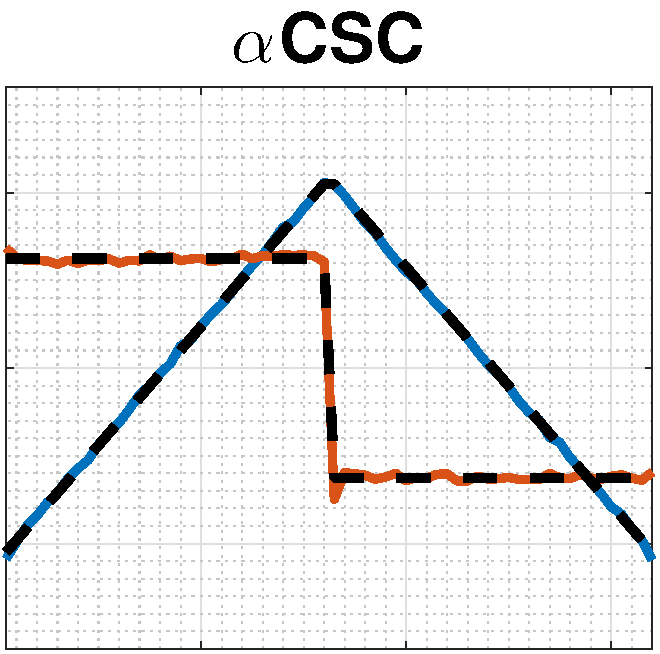
\includegraphics[width=\tmpsize\linewidth]{figures/synth_1_2_v2.pdf}
        \end{tabular}
} \hfill
\subfigure[10\% corruption. ]{
\setlength{\tabcolsep}{0.5pt} 
\begin{tabular}{c c}
        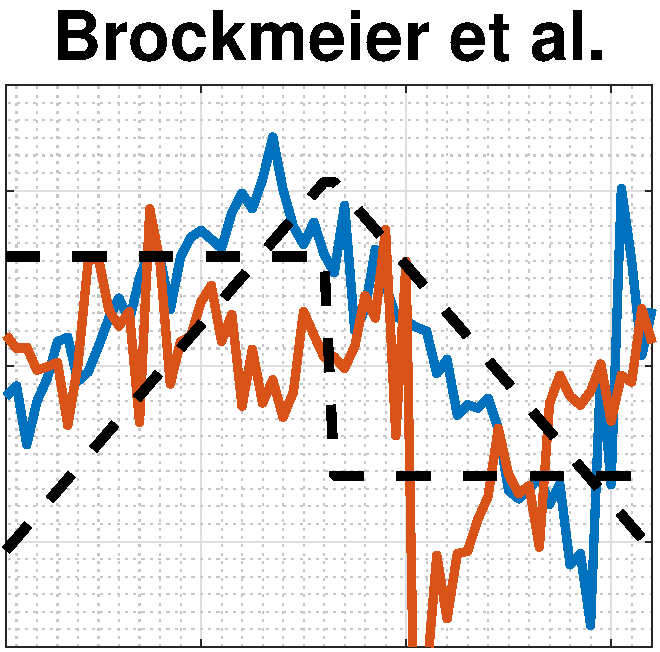
\includegraphics[width=\tmpsize\linewidth]{figures/synth_2_rnn_v2.pdf} &
        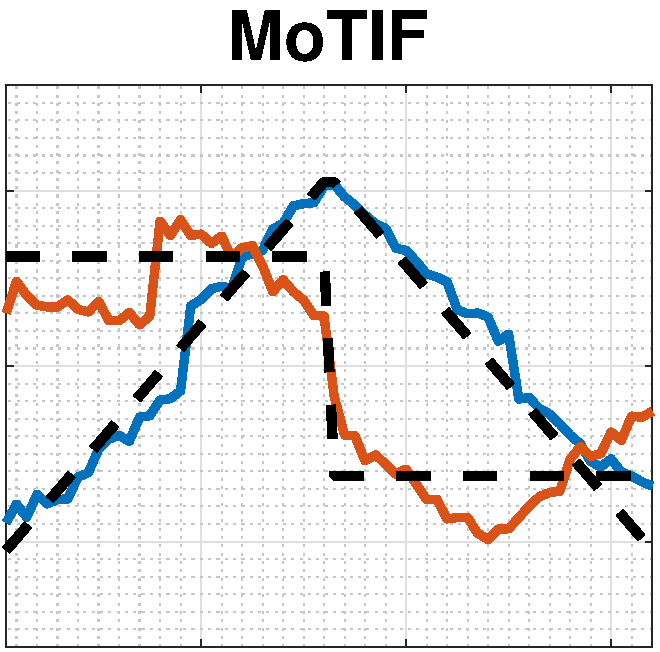
\includegraphics[width=\tmpsize\linewidth]{figures/synth_2_motif_v2.pdf}
\\
        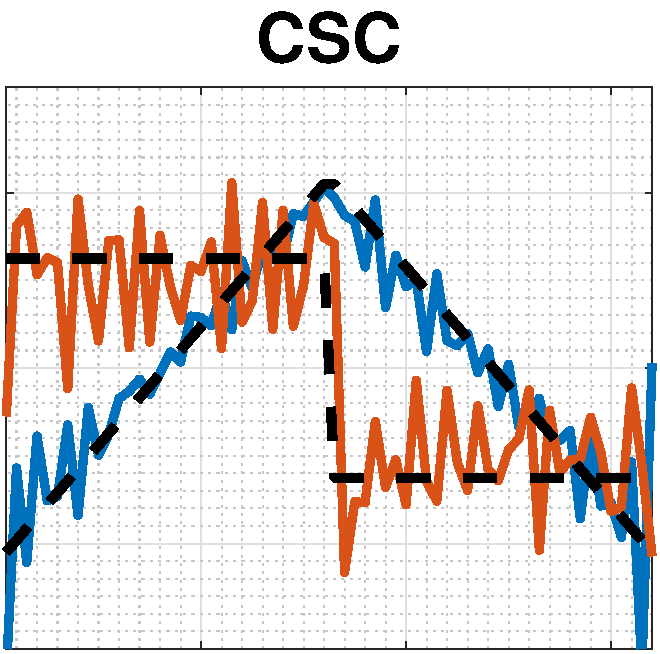
\includegraphics[width=\tmpsize\linewidth]{figures/synth_2_1_v2.pdf} &
        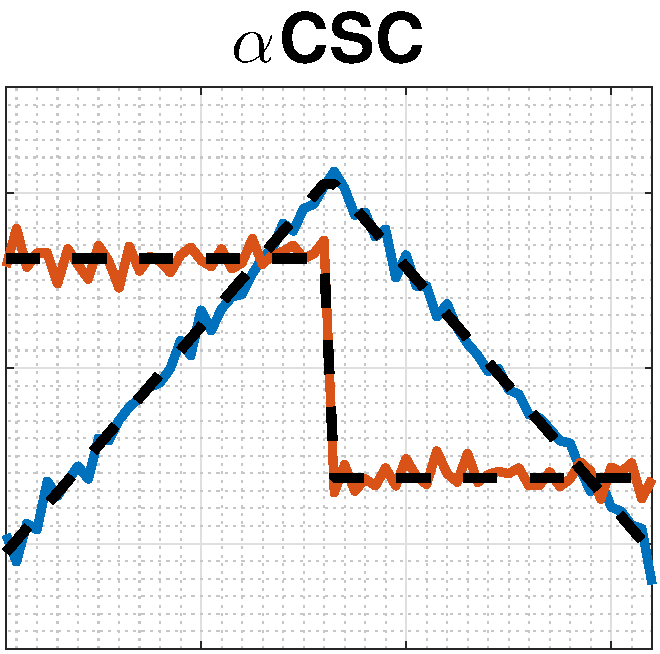
\includegraphics[width=\tmpsize\linewidth]{figures/synth_2_2_v2.pdf}
        \end{tabular}
}\hfill
\subfigure[20\% corruption]{
\setlength{\tabcolsep}{0.5pt} 
\begin{tabular}{c c}
    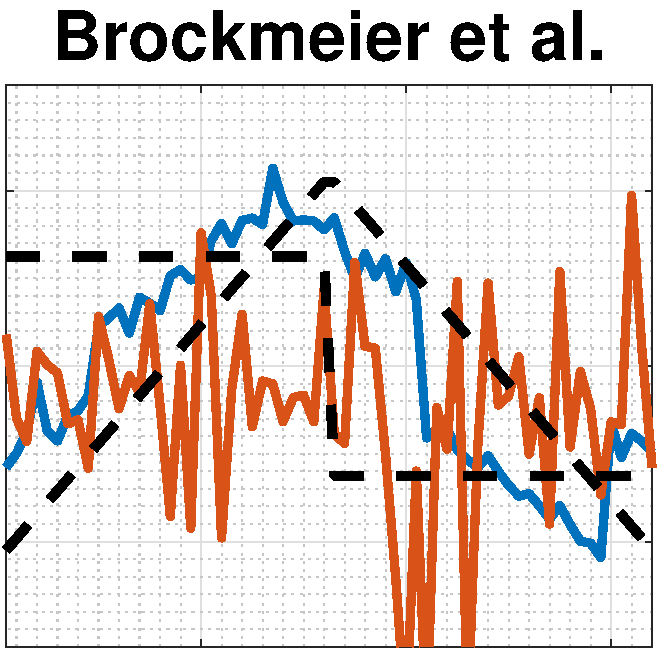
\includegraphics[width=\tmpsize\linewidth]{figures/synth_3_rnn_v2.pdf} & 
    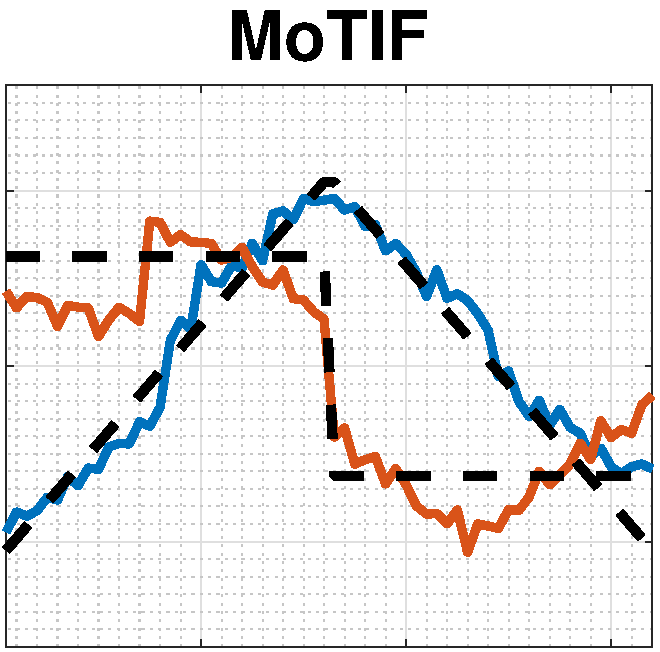
\includegraphics[width=\tmpsize\linewidth]{figures/synth_3_motif_v2.pdf}\\
%
    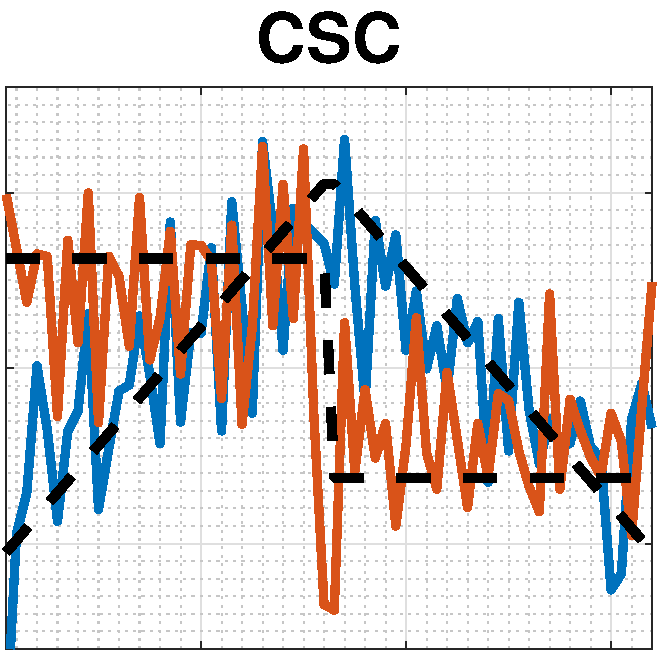
\includegraphics[width=\tmpsize\linewidth]{figures/synth_3_1_v2.pdf}&
    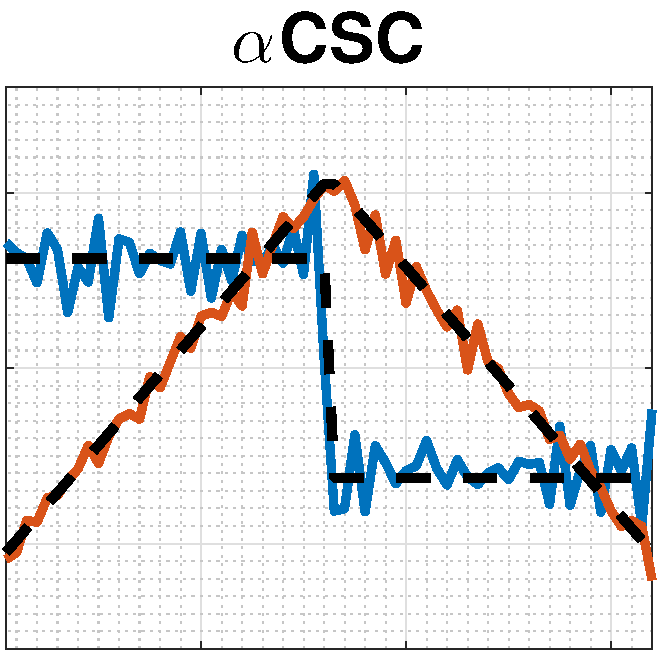
\includegraphics[width=\tmpsize\linewidth]{figures/synth_3_2_v2.pdf}
    \end{tabular}
}
\end{center}
\vspace{-15pt}
\caption[Simulation to compare state-of-the-art methods against $\alpha$CSC.]{Simulation to compare state-of-the-art methods against $\alpha$CSC.}
\label{fig:mcem_simulated} 
\vspace{-10pt}
\end{figure}
%
%
%%%%%%%%%%%%%%%%%%%%%%%%%%%%%%%%%%%%%%%%%%%%%%%%%%%%%%%%%%%%%%%
%%%%%%%%%%%%%%%%%%%%%%%%%%%%%%%%%%%%%%%%%%%%%%%%%%%%%%%%%%%%%%%
%
% \paragraph{Robustness against corrupted data:}
%


\textbf{Robustness to corrupted data:} 
In our second synthetic data experiment, we illustrate the robustness of $\alpha$CSC in the presence of corrupted observations.
%
In order to simulate the likely presence of high amplitude artifacts, one way would be to directly simulate the generative model in \eqref{eqn:acsc_org}. However, this would give us an unfair advantage, since $\alpha$CSC is specifically designed for such data. Here, we take an alternative approach, where we corrupt a randomly chosen fraction of the trials ($10\%$ or $20\%$) with strong Gaussian noise of standard deviation $0.1$, \textit{i.e.} one order of magnitude higher than in a regular trial. We used a regularization parameter of $\lambda = 0.1$.
%
In these experiments, by CSC we refer to $\alpha$CSC with $\alpha=2$, that resembles using only the M-step of our algorithm with deterministic weights $w_{n,t}=1/2$ for all $n$, $t$. We used a simpler setup where we set $N=100$, $T=512$, and $L=64$. We used $K=2$ atoms, as shown in dashed lines in Fig.~\ref{fig:mcem_simulated}.

% We test the standard CSC and $\alpha$CSC algorithms on the simulated data corrupted with artifacts.
%
 %~\footnote{For the CSC model it matches atoms that lead to the smallest values of the objective.}.

% The reader may have already noticed that computing this is not possible when working with real data because the true atoms are not known. Indeed, when multiple restarts are involved, the best restart can be chosen only if one is minimizing a well-defined cost function.
%
For $\alpha$CSC, we set the number of outer iterations $I=5$, the number of iterations of the M-step to $M=50$, and the number of iterations of the MCMC algorithm to $J=10$. We discard the first $5$ samples of the MCMC algorithm as burn-in.
%
% We set $I=5$ iterations of the EM algorithm in $\alpha$CSC and , starting with the M-step and ending with the M-step. The MCMC algorithm was run for 10 iterations with the first 5 iterations being discarded for computing the expectation. 
%
To enable a fair comparison, we run the standard CSC algorithm for $I\times M$ iterations, i.e.\ the \emph{total} number of M-step iterations in $\alpha$CSC. We also compared $\alpha$CSC against competing state-of-art methods previously applied to neural time series: \citet{brockmeier2016learning} and MoTIF~\cite{jost2006motif}. 
%
Starting from multiple random initializations, the estimated atoms with the smallest $\ell_2$ distance with the true atoms are shown in Fig.~\ref{fig:mcem_simulated}.

% The learned atoms are shown in Fig.~\ref{fig:mcem_simulated}. 

\begin{figure}[b]
    \centering
    \begin{minipage}{\linewidth}
        \begin{minipage}{0.75\textwidth}
             \subfigure[LFP spike data from \cite{hitziger2017adaptive}]{
             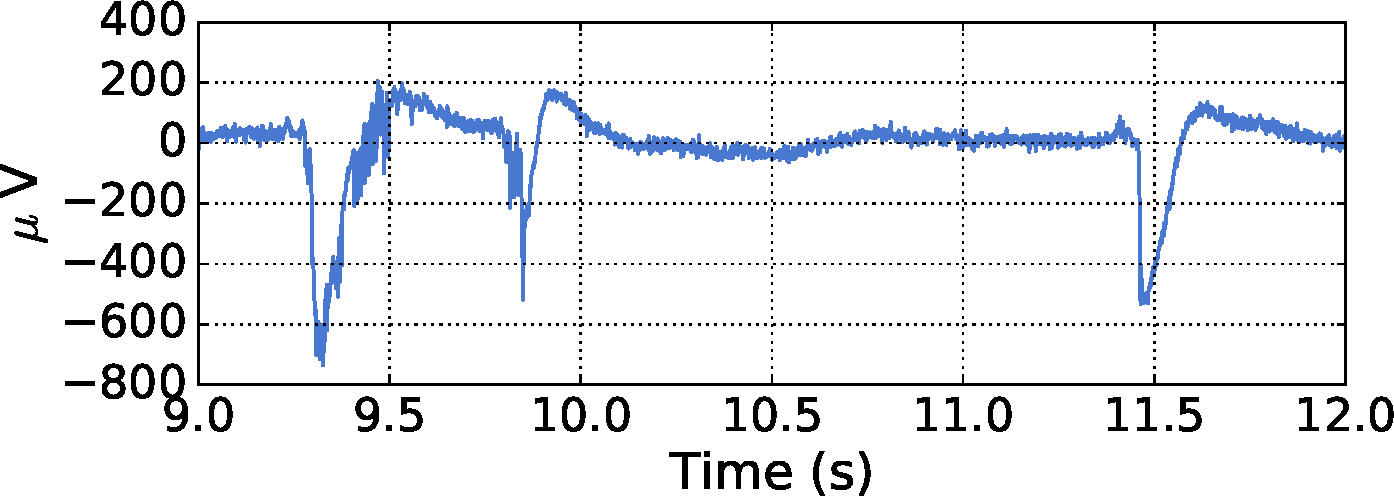
\includegraphics[height=2.3cm]{figures/spike_atomsa.pdf}
             \label{fig:spikedata}}
             \subfigure[Estimated atoms]{
             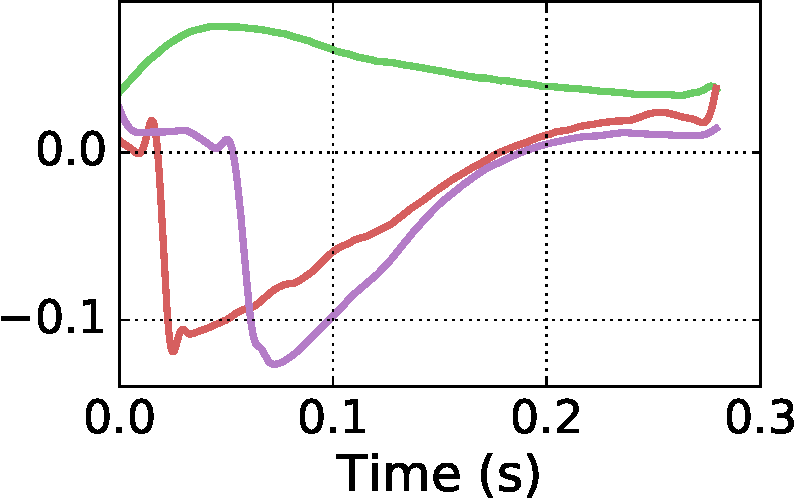
\includegraphics[height=2.2cm]{figures/spike_atomsb.pdf}
             \label{fig:spikeatoms}}
        \end{minipage}
        \hfill
        \begin{minipage}{0.23\textwidth}
            \caption[Atoms learnt by $\alpha$CSC on LFP data containing epileptiform spikes with $\alpha=2$.]{Atoms learnt by $\alpha$CSC on LFP data containing epileptiform spikes with $\alpha=2$.}
        \end{minipage}
    % \vspace{-10pt}
    \end{minipage}
\end{figure}

In the artifact-free scenario, all algorithms perform equally well, except for MoTIF that suffers from the presence of activations with varying amplitudes. This is because it aligns the data using correlations before performing the eigenvalue decomposition, without taking into account the strength of activations in each trial. The performance of \citet{brockmeier2016learning} and CSC degrades as the level of corruption increases. On the other hand, $\alpha$CSC is clearly more robust to the increasing level of corruption and recovers reasonable atoms even when 20\% of the trials are corrupted. 



% $\alpha$CSC learned good atoms even on corrupted data.

\textbf{Results on LFP data}
In our last set of experiments, we consider real neural data from two different datasets. 
%
We first applied $\alpha$CSC on an LFP dataset previously used in~\cite{hitziger2017adaptive} and containing epileptiform spikes as shown in Fig.~\ref{fig:spikedata}. The data was recorded in the rat cortex, and  is free of artifact. Therefore, we used the standard CSC with our optimization scheme, (i.e.\ $\alpha$CSC with $\alpha=2$).
%
As a standard preprocessing procedure, we applied a high-pass filter at $1$\,Hz in order to remove drifts in the signal, and then applied a tapered cosine window to down-weight the samples near the edges. We set $\lambda=6$, $N=300$, $T=2500$, $L=350$, and $K=3$. The recovered atoms by our algorithm are shown in Fig.~\ref{fig:spikeatoms}. We can observe that the estimated atoms resemble the spikes in Fig.~\ref{fig:spikedata}. These results show that, without using any heuristics, our approach can recover similar atoms to the ones reported in \cite{hitziger2017adaptive}, even though it does not make any assumptions on the shapes of the waveforms, or initializes the atoms with template spikes in order to ease the optimization.


% Interpreting these atoms is not so straightforward, however it is easy to verify visually these atoms resemble the spikes in Fig.~\ref{fig:spikedata}.



The second dataset is an LFP channel in a rodent striatum from~\cite{dallerac2017updating}. We segmented the data into $70$ trials of length $2500$ samples, windowed each trial with a tapered cosine function, and detrended the data with a high-pass filter at $1$\,Hz.
 % to downweight the effect of samples near the edges, which cannot be handled gracefully by the convolutions. 
We set $\lambda=10$, initialized the weights $w_n$ to the inverse of the variance of the trial $x_n$. Atoms are in all experiments initialized with Gaussian white noise.


% We compared $\alpha$CSC against CSC on artifact-free data and on data corrupted by strong artifacts (see Fig.~\ref{fig:pdf_lfp}). 

As opposed to the first LFP dataset, this dataset contains strong artifacts, as shown in Fig.~\ref{fig:artifacts}. In order to be able to illustrate the potential of CSC on this data, we first \emph{manually} identified and removed the trials that were corrupted by artifacts. In Fig.~\ref{fig:rat3atoms}, we illustrate the estimated atoms with CSC on the manually-cleaned data. We observe that the estimated atoms correspond to canonical waveforms found in the signal. In particular, the high frequency oscillations around $80$\,Hz are modulated in amplitude by the low-frequency oscillation around $3$\,Hz, a phenomenon known as cross-frequency coupling (CFC)~\cite{jensen2007cross}. We can observe this by computing a comodulogram~\cite{tort2010measuring} on the entire signal (Fig.~\ref{fig:comodulogram}). This measures the correlation between the amplitude of the high frequency band and the phase of the low frequency band. 


Even though CSC is able to provide these excellent results on the cleaned data set, its performance heavily relies on the manual removal of the artifacts. Finally, we repeated the previous experiment on the full data, without removing the artifacts and compared CSC with $\alpha$CSC, where we set $\alpha=1.2$. The results are shown in the middle and the right sub-figures of Fig.~\ref{fig:rat3atoms}. It can be observed that in the presence of strong artifacts, CSC is not able to recover the atoms anymore. On the contrary, we observe that $\alpha$CSC can still recover atoms as observed in the artifact-free regime. In particular, the cross-frequency coupling phenomenon is still visible.


\begin{figure}[t]
    \centering
    \subfigure[Atoms learnt by: CSC (clean data), CSC (full data), $\alpha$CSC (full data)]{
    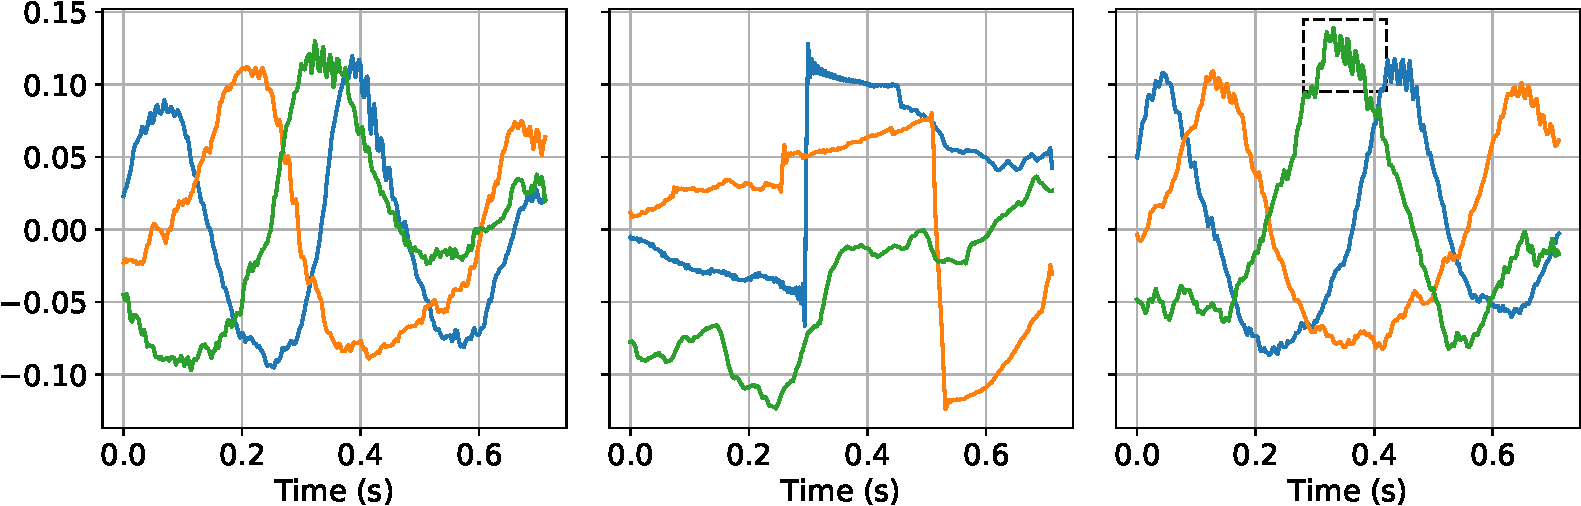
\includegraphics[width=0.65\linewidth]{figures/rat3atoms.pdf}
    \label{fig:rat3atoms}
    }
    \subfigure[Comodulogram.]{
    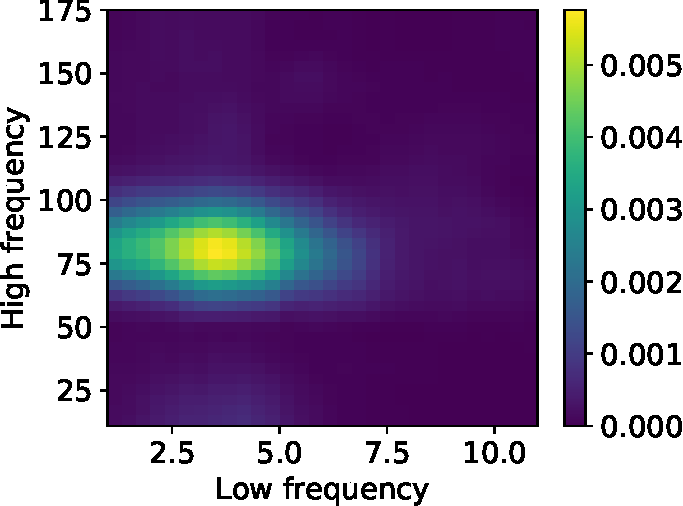
\includegraphics[width=0.28\linewidth]{figures/comodulogram.pdf}
    \label{fig:comodulogram}
    }
    \vspace{-10pt}
    \caption[Three atoms learnt from a rodent striatal LFP channel, using CSC on cleaned data, and both CSC and $\alpha$CSC on the full data.]{(a)~Three atoms learnt from a rodent striatal LFP channel, using CSC on cleaned data, and both CSC and $\alpha$CSC on the full data. The atoms capture the cross-frequency coupling of the data (dashed rectangle). (b)~Comodulogram presents the cross-frequency coupling intensity computed between pairs of frequency bands on the entire cleaned signal, following \cite{tort2010measuring}.}
    \label{fig:ratdata}
    \vspace{-10pt}
\end{figure}


  % However, when the data contains heavy artifacts, . Indeed, to recover the prototypical atoms in the presence of artifacts, we must use $\alpha$CSC as shown in the last subplot of .

%) are good when the data is artifact-free, but are strongly affected by the artifacts. On the contrary, the atoms learned with $\alpha$CSC are also good on corrupted data. Interestingly, we are able to recover from the data not only the triangular shaped oscillation, but also the \emph{cross-frequency coupling}. Indeed, in this signal, the high frequency oscillations around 80\,Hz are modulated in amplitude by the low-frequency oscillation around 3\,Hz.
%To visualize this cross-frequency coupling, we computed a comodulogram on the entire signal (Fig.~\ref{fig:comodulogram}). For each pairs of frequency bands, it quantifies the correlation between the amplitude of the high frequency and the phase of the low frequency, following the method from \cite{tort2010measuring}.
%The three atoms all capture this cross-frequency coupling, and show different canonical shapes for the signal.

